\documentclass[12pt]{article}
\usepackage[english]{babel}
\usepackage[utf8]{inputenc}
\usepackage{amsmath, amssymb, amsthm}
\usepackage{graphicx}
\usepackage{hyperref}
\usepackage{geometry}
\usepackage{xcolor}
\usepackage{tikz}

\setlength{\topmargin}{0pt}
\setlength{\headsep}{0pt}
\textheight = 600pt

\title{Graph Theory \\ Homework 2}
\author{Ben Kallus and Maddy LaPoint}
\date{Due Monday, February 15}

\begin{document}
\pagecolor{black}
\color{white}
\maketitle

\noindent{\bf 1.23}

{\bf (a)} For $k=1$, the following graph satisfies the condition:

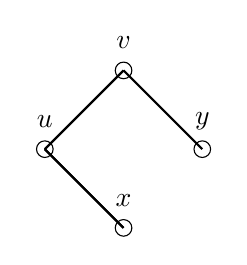
\begin{tikzpicture}
\draw[fill=white] (1.0, 0.0) circle (3pt);
\draw[fill=white] (0.0, 1.0) circle (3pt);
\draw[fill=white] (-1.0, 0.0) circle (3pt);
\draw[fill=white] (-0.0, -1.0) circle (3pt);

\node at (1.0,0.35) {$y$};
\node at (0.0,1.35) {$v$};
\node at (-1.0,0.35) {$u$};
\node at (-0.0,-.65) {$x$};

\draw[thick] (1.0, 0.0) -- (0.0, 1.0);
\draw[thick] (0.0, 1.0) -- (-1.0, 0.0);
\draw[thick] (-1.0, 0.0) -- (-0.0, -1.0);
\draw[thick] (-0.0, -1.0) -- (-1.0, 0.0);
\end{tikzpicture}

\medskip
For $k=2$, the following graph satisfies the condition:

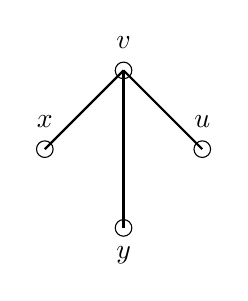
\begin{tikzpicture}
\draw[fill=white] (1.0, 0.0) circle (3pt);
\node at (1.0, 0.35) {$u$};
\draw[fill=white] (0.0, 1.0) circle (3pt);
\node at (0.0, 1.35) {$v$};
\draw[fill=white] (-1.0, 0.0) circle (3pt);
\node at (-1.0, 0.35) {$x$};
\draw[fill=white] (-0.0, -1.0) circle (3pt);
\node at (0.0, -1.35) {$y$};

\draw[thick] (1.0, 0.0) -- (0.0, 1.0);
\draw[thick] (0.0, 1.0) -- (-0.0, -1.0);
\draw[thick] (-1.0, 0.0) -- (0.0, 1.0);
\draw[thick] (-0.0, -1.0) -- (0.0, 1.0);
\end{tikzpicture}

{\bf (b)} Observe that the following graph satisfies the condition for $k=3$:

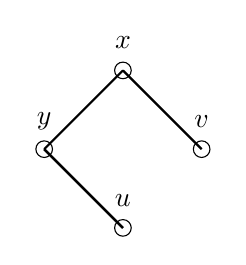
\begin{tikzpicture}
\draw[fill=white] (1.0, 0.0) circle (3pt);
\draw[fill=white] (0.0, 1.0) circle (3pt);
\draw[fill=white] (-1.0, 0.0) circle (3pt);
\draw[fill=white] (-0.0, -1.0) circle (3pt);

\node at (1.0,0.35) {$v$};
\node at (0.0,1.35) {$x$};
\node at (-1.0,0.35) {$y$};
\node at (-0.0,-.65) {$u$};

\draw[thick] (1.0, 0.0) -- (0.0, 1.0);
\draw[thick] (0.0, 1.0) -- (-1.0, 0.0);
\draw[thick] (-1.0, 0.0) -- (-0.0, -1.0);
\draw[thick] (-0.0, -1.0) -- (-1.0, 0.0);
\end{tikzpicture}

\medskip
{\bf Proposition:} 3 is the largest value of $k$ for which the answer to the question is "yes".
\begin{proof}
    Let $G$ be a connected graph whose complement is also connected.
    Suppose, toward a contradiction, that $G$ contains four distinct vertices $u,v,x,y$ such that $d_G(u,v) = 4 = d_{\overline{G}}(x,y)$.
    Then, there exists a $u-v$ geodesic $P = (u = p_0, p_1, p_2, p_3 = v)$ in $G$, and a $x-y$ geodesic $Q = (x = q_0, q_1, q_2, q_3 = y)$ in $\overline G$.
    FINISH ME!!!!!!!
\end{proof}

\bigskip
\noindent{\bf 1.25}

{\bf Proposition:} Let $G$ be a connected graph of order 5 or more. Then, at most one of $G$ and $\overline G$ is bipartite.
\begin{proof}
    Let $G$ be a connected, bipartite graph of order 5 or more.
    Let $a$, $b$, and $c$ be three distinct vertices in one of $G$'s partite sets.
    Note that such vertices are guaranteed to exist, since 5 cannot be split into 2 nonnegative integer parts both less than 3.
    Since $a$, $b$, and $c$ are in the same partite set in $G$, there must be no edges between them in $G$.
    Thus, $a$, $b$, and $c$ must be a clique in $\overline G$.
    Thus, $\overline G$ contains the odd cycle $(a,b,c)$.
    Therefore, by Theorem 1.12, $\overline G$ is not bipartite.
    Thus, at most one of $G$ and $\overline G$ can be bipartite.
\end{proof}

\bigskip
\noindent{\bf 1.27}

\noindent{\bf (a)} $K_5 + K_2:$

\medskip
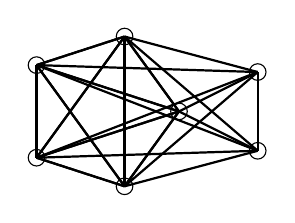
\begin{tikzpicture}
\draw[fill=white] (1.0, 0.0) circle (3pt);
\draw[fill=white] (0.309, 0.951) circle (3pt);
\draw[fill=white] (-0.809, 0.588) circle (3pt);
\draw[fill=white] (-0.809, -0.588) circle (3pt);
\draw[fill=white] (0.309, -0.951) circle (3pt);
\draw[fill=white] (2, .5) circle (3pt);
\draw[fill=white] (2, -.5) circle (3pt);

\draw[thick] (1.0, 0.0) -- (0.309, -0.951);
\draw[thick] (1.0, 0.0) -- (0.309, 0.951);
\draw[thick] (1.0, 0.0) -- (-0.809, 0.588);
\draw[thick] (1.0, 0.0) -- (-0.809, -0.588);
\draw[thick] (0.309, 0.951) -- (1.0, 0.0);
\draw[thick] (0.309, 0.951) -- (-0.809, -0.588);
\draw[thick] (0.309, 0.951) -- (0.309, -0.951);
\draw[thick] (0.309, 0.951) -- (-0.809, 0.588);
\draw[thick] (-0.809, 0.588) -- (1.0, 0.0);
\draw[thick] (-0.809, 0.588) -- (0.309, 0.951);
\draw[thick] (-0.809, 0.588) -- (0.309, -0.951);
\draw[thick] (-0.809, 0.588) -- (-0.809, -0.588);
\draw[thick] (-0.809, -0.588) -- (1.0, 0.0);
\draw[thick] (-0.809, -0.588) -- (0.309, 0.951);
\draw[thick] (-0.809, -0.588) -- (0.309, -0.951);
\draw[thick] (-0.809, -0.588) -- (-0.809, 0.588);
\draw[thick] (0.309, -0.951) -- (1.0, 0.0);
\draw[thick] (0.309, -0.951) -- (0.309, 0.951);
\draw[thick] (0.309, -0.951) -- (-0.809, 0.588);
\draw[thick] (0.309, -0.951) -- (-0.809, -0.588);
\draw[thick] (2, .5) -- (2, -.5);
\draw[thick](1.0, 0.0) -- (2, .5);
\draw[thick](0.309, 0.951) -- (2, .5);
\draw[thick](-0.809, 0.588) -- (2, .5);
\draw[thick](-0.809, -0.588) -- (2, .5);
\draw[thick](0.309, -0.951) -- (2, .5);
\draw[thick](1.0, 0.0) -- (2, -.5);
\draw[thick](0.309, 0.951) -- (2, -.5);
\draw[thick](-0.809, 0.588) -- (2, -.5);
\draw[thick](-0.809, -0.588) -- (2, -.5);
\draw[thick](0.309, -0.951) -- (2, -.5);
\end{tikzpicture}

\medskip
$K_5 \times K_2$:

\medskip
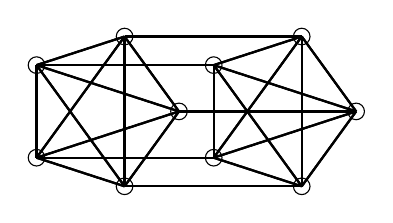
\begin{tikzpicture}
\draw[fill=white] (1.0, 0.0) circle (3pt);
\draw[fill=white] (0.309, 0.951) circle (3pt);
\draw[fill=white] (-0.809, 0.588) circle (3pt);
\draw[fill=white] (-0.809, -0.588) circle (3pt);
\draw[fill=white] (0.309, -0.951) circle (3pt);

\draw[thick] (1.0, 0.0) -- (0.309, -0.951);
\draw[thick] (1.0, 0.0) -- (0.309, 0.951);
\draw[thick] (1.0, 0.0) -- (-0.809, 0.588);
\draw[thick] (1.0, 0.0) -- (-0.809, -0.588);
\draw[thick] (0.309, 0.951) -- (1.0, 0.0);
\draw[thick] (0.309, 0.951) -- (-0.809, -0.588);
\draw[thick] (0.309, 0.951) -- (0.309, -0.951);
\draw[thick] (0.309, 0.951) -- (-0.809, 0.588);
\draw[thick] (-0.809, 0.588) -- (1.0, 0.0);
\draw[thick] (-0.809, 0.588) -- (0.309, 0.951);
\draw[thick] (-0.809, 0.588) -- (0.309, -0.951);
\draw[thick] (-0.809, 0.588) -- (-0.809, -0.588);
\draw[thick] (-0.809, -0.588) -- (1.0, 0.0);
\draw[thick] (-0.809, -0.588) -- (0.309, 0.951);
\draw[thick] (-0.809, -0.588) -- (0.309, -0.951);
\draw[thick] (-0.809, -0.588) -- (-0.809, 0.588);
\draw[thick] (0.309, -0.951) -- (1.0, 0.0);
\draw[thick] (0.309, -0.951) -- (0.309, 0.951);
\draw[thick] (0.309, -0.951) -- (-0.809, 0.588);
\draw[thick] (0.309, -0.951) -- (-0.809, -0.588);

\draw[fill=white] (2.25+1.0, 0.0) circle (3pt);
\draw[fill=white] (2.25+0.309, 0.951) circle (3pt);
\draw[fill=white] (2.25+-0.809, 0.588) circle (3pt);
\draw[fill=white] (2.25+-0.809, -0.588) circle (3pt);
\draw[fill=white] (2.25+0.309, -0.951) circle (3pt);

\draw[thick] (2.25+1.0, 0.0) -- (2.25+0.309, -0.951);
\draw[thick] (2.25+1.0, 0.0) -- (2.25+0.309, 0.951);
\draw[thick] (2.25+1.0, 0.0) -- (2.25+-0.809, 0.588);
\draw[thick] (2.25+1.0, 0.0) -- (2.25+-0.809, -0.588);
\draw[thick] (2.25+0.309, 0.951) -- (2.25+1.0, 0.0);
\draw[thick] (2.25+0.309, 0.951) -- (2.25+-0.809, -0.588);
\draw[thick] (2.25+0.309, 0.951) -- (2.25+0.309, -0.951);
\draw[thick] (2.25+0.309, 0.951) -- (2.25+-0.809, 0.588);
\draw[thick] (2.25+-0.809, 0.588) -- (2.25+1.0, 0.0);
\draw[thick] (2.25+-0.809, 0.588) -- (2.25+0.309, 0.951);
\draw[thick] (2.25+-0.809, 0.588) -- (2.25+0.309, -0.951);
\draw[thick] (2.25+-0.809, 0.588) -- (2.25+-0.809, -0.588);
\draw[thick] (2.25+-0.809, -0.588) -- (2.25+1.0, 0.0);
\draw[thick] (2.25+-0.809, -0.588) -- (2.25+0.309, 0.951);
\draw[thick] (2.25+-0.809, -0.588) -- (2.25+0.309, -0.951);
\draw[thick] (2.25+-0.809, -0.588) -- (2.25+-0.809, 0.588);
\draw[thick] (2.25+0.309, -0.951) -- (2.25+1.0, 0.0);
\draw[thick] (2.25+0.309, -0.951) -- (2.25+0.309, 0.951);
\draw[thick] (2.25+0.309, -0.951) -- (2.25+-0.809, 0.588);
\draw[thick] (2.25+0.309, -0.951) -- (2.25+-0.809, -0.588);

\draw[thick] (1.0, 0.0) -- (2.25+1.0, 0.0);
\draw[thick] (2.25+0.309, 0.951) -- (0.309, 0.951);
\draw[thick] (2.25+-0.809, 0.588) -- (-0.809, 0.588);
\draw[thick] (-0.809, -0.588) -- (2.25+-0.809, -0.588);
\draw[thick] (0.309, -0.951) -- (2.25+0.309, -0.951);
\end{tikzpicture}

\bigskip
\noindent{\bf (b)} $\overline{K_5} + \overline{K_3}$:

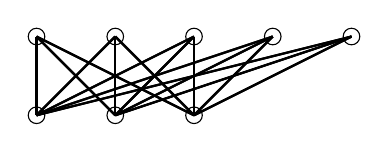
\begin{tikzpicture}
\draw[fill=white] (0, 0) circle (3pt);
\draw[fill=white] (0, 1) circle (3pt);
\draw[fill=white] (1, 1) circle (3pt);
\draw[fill=white] (2, 1) circle (3pt);
\draw[fill=white] (3, 1) circle (3pt);
\draw[fill=white] (4, 1) circle (3pt);
\draw[fill=white] (1, 0) circle (3pt);
\draw[fill=white] (2, 0) circle (3pt);

\draw[thick] (0, 0) -- (4, 1);
\draw[thick] (0, 0) -- (1, 1);
\draw[thick] (0, 0) -- (2, 1);
\draw[thick] (0, 0) -- (0, 1);
\draw[thick] (0, 0) -- (3, 1);
\draw[thick] (0, 1) -- (0, 0);
\draw[thick] (0, 1) -- (1, 0);
\draw[thick] (0, 1) -- (2, 0);
\draw[thick] (1, 1) -- (0, 0);
\draw[thick] (1, 1) -- (1, 0);
\draw[thick] (1, 1) -- (2, 0);
\draw[thick] (2, 1) -- (0, 0);
\draw[thick] (2, 1) -- (1, 0);
\draw[thick] (2, 1) -- (2, 0);
\draw[thick] (3, 1) -- (0, 0);
\draw[thick] (3, 1) -- (1, 0);
\draw[thick] (3, 1) -- (2, 0);
\draw[thick] (4, 1) -- (0, 0);
\draw[thick] (4, 1) -- (1, 0);
\draw[thick] (4, 1) -- (2, 0);
\draw[thick] (1, 0) -- (4, 1);
\draw[thick] (1, 0) -- (1, 1);
\draw[thick] (1, 0) -- (2, 1);
\draw[thick] (1, 0) -- (0, 1);
\draw[thick] (1, 0) -- (3, 1);
\draw[thick] (2, 0) -- (4, 1);
\draw[thick] (2, 0) -- (1, 1);
\draw[thick] (2, 0) -- (2, 1);
\draw[thick] (2, 0) -- (0, 1);
\draw[thick] (2, 0) -- (3, 1);
\end{tikzpicture}

\medskip
$\overline{K_5} \times \overline{K_3}$:

\medskip
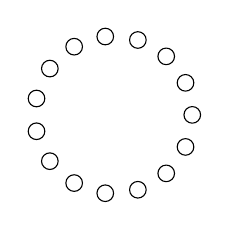
\begin{tikzpicture}
\draw[fill=white] (1.0, 0.0) circle (3pt);
\draw[fill=white] (0.914, 0.407) circle (3pt);
\draw[fill=white] (0.669, 0.743) circle (3pt);
\draw[fill=white] (0.309, 0.951) circle (3pt);
\draw[fill=white] (-0.105, 0.995) circle (3pt);
\draw[fill=white] (-0.5, 0.866) circle (3pt);
\draw[fill=white] (-0.809, 0.588) circle (3pt);
\draw[fill=white] (-0.978, 0.208) circle (3pt);
\draw[fill=white] (-0.978, -0.208) circle (3pt);
\draw[fill=white] (-0.809, -0.588) circle (3pt);
\draw[fill=white] (-0.5, -0.866) circle (3pt);
\draw[fill=white] (-0.105, -0.995) circle (3pt);
\draw[fill=white] (0.309, -0.951) circle (3pt);
\draw[fill=white] (0.669, -0.743) circle (3pt);
\draw[fill=white] (0.914, -0.407) circle (3pt);
\end{tikzpicture}

\newpage
\noindent{\bf (c)} $C_5 + K_1$:

\medskip
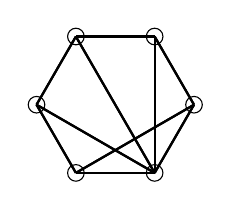
\begin{tikzpicture}
\draw[fill=white] (1.0, 0.0) circle (3pt);
\draw[fill=white] (0.5, 0.866) circle (3pt);
\draw[fill=white] (-0.5, 0.866) circle (3pt);
\draw[fill=white] (-1.0, 0.0) circle (3pt);
\draw[fill=white] (-0.5, -0.866) circle (3pt);
\draw[fill=white] (0.5, -0.866) circle (3pt);

\draw[thick] (1.0, 0.0) -- (0.5, 0.866);
\draw[thick] (1.0, 0.0) -- (0.5, -0.866);
\draw[thick] (1.0, 0.0) -- (-0.5, -0.866);
\draw[thick] (0.5, 0.866) -- (1.0, 0.0);
\draw[thick] (0.5, 0.866) -- (0.5, -0.866);
\draw[thick] (0.5, 0.866) -- (-0.5, 0.866);
\draw[thick] (-0.5, 0.866) -- (0.5, 0.866);
\draw[thick] (-0.5, 0.866) -- (0.5, -0.866);
\draw[thick] (-0.5, 0.866) -- (-1.0, 0.0);
\draw[thick] (-1.0, 0.0) -- (-0.5, -0.866);
\draw[thick] (-1.0, 0.0) -- (0.5, -0.866);
\draw[thick] (-1.0, 0.0) -- (-0.5, 0.866);
\draw[thick] (-0.5, -0.866) -- (1.0, 0.0);
\draw[thick] (-0.5, -0.866) -- (0.5, -0.866);
\draw[thick] (-0.5, -0.866) -- (-1.0, 0.0);
\draw[thick] (0.5, -0.866) -- (0.5, 0.866);
\draw[thick] (0.5, -0.866) -- (-0.5, 0.866);
\draw[thick] (0.5, -0.866) -- (1.0, 0.0);
\draw[thick] (0.5, -0.866) -- (-1.0, 0.0);
\draw[thick] (0.5, -0.866) -- (-0.5, -0.866);
\end{tikzpicture}

\medskip
$C_5 \times K_1$:

\medskip
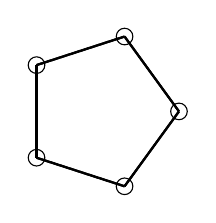
\begin{tikzpicture}
\draw[fill=white] (1.0, 0.0) circle (3pt);
\draw[fill=white] (0.309, 0.951) circle (3pt);
\draw[fill=white] (-0.809, 0.588) circle (3pt);
\draw[fill=white] (-0.809, -0.588) circle (3pt);
\draw[fill=white] (0.309, -0.951) circle (3pt);

\draw[thick] (1.0, 0.0) -- (0.309, 0.951);
\draw[thick] (1.0, 0.0) -- (0.309, -0.951);
\draw[thick] (0.309, 0.951) -- (-0.809, 0.588);
\draw[thick] (0.309, 0.951) -- (1.0, 0.0);
\draw[thick] (-0.809, 0.588) -- (0.309, 0.951);
\draw[thick] (-0.809, 0.588) -- (-0.809, -0.588);
\draw[thick] (-0.809, -0.588) -- (-0.809, 0.588);
\draw[thick] (-0.809, -0.588) -- (0.309, -0.951);
\draw[thick] (0.309, -0.951) -- (-0.809, -0.588);
\draw[thick] (0.309, -0.951) -- (1.0, 0.0);
\end{tikzpicture}

{\bf 1.28}

\noindent{\bf (a)} $R_2$:

\medskip
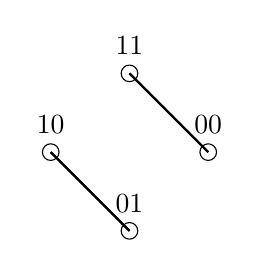
\begin{tikzpicture}
\draw[fill=white] (1.0, 0.0) circle (3pt);
\node at (1.0, 0.35) {00};
\draw[fill=white] (0.0, 1.0) circle (3pt);
\node at (0.0, 1.35) {11};
\draw[fill=white] (-1.0, 0.0) circle (3pt);
\node at (-1.0, 0.35) {10};
\draw[fill=white] (-0.0, -1.0) circle (3pt);
\node at (0.0, -0.65) {01};

\draw[thick] (1.0, 0.0) -- (0.0, 1.0);
\draw[thick] (0.0, 1.0) -- (1.0, 0.0);
\draw[thick] (-1.0, 0.0) -- (-0.0, -1.0);
\draw[thick] (-0.0, -1.0) -- (-1.0, 0.0);
\end{tikzpicture}

\medskip
$R_3$:

\medskip
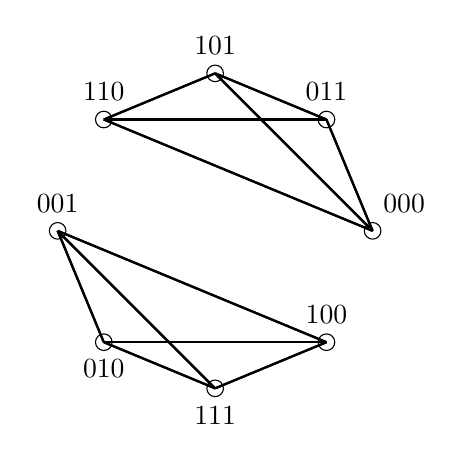
\begin{tikzpicture}
\draw[fill=white] (2.0, 0.0) circle (3pt);
\node at (2.4, 0.35) {000};
\draw[fill=white] (1.414, 1.414) circle (3pt);
\node at (1.414, 1.7639999999999998) {011};
\draw[fill=white] (0.0, 2.0) circle (3pt);
\node at (0.0, 2.35) {101};
\draw[fill=white] (-1.414, 1.414) circle (3pt);
\node at (-1.414, 1.7639999999999998) {110};
\draw[fill=white] (-2.0, 0.0) circle (3pt);
\node at (-2.0, 0.35) {001};
\draw[fill=white] (-1.414, -1.414) circle (3pt);
\node at (-1.414, -1.75) {010};
\draw[fill=white] (-0.0, -2.0) circle (3pt);
\node at (0.0, -2.35) {111};
\draw[fill=white] (1.414, -1.414) circle (3pt);
\node at (1.414, -1.064) {100};

\draw[thick] (2.0, 0.0) -- (1.414, 1.414);
\draw[thick] (2.0, 0.0) -- (0.0, 2.0);
\draw[thick] (2.0, 0.0) -- (-1.414, 1.414);
\draw[thick] (1.414, 1.414) -- (0.0, 2.0);
\draw[thick] (1.414, 1.414) -- (-1.414, 1.414);
\draw[thick] (1.414, 1.414) -- (2.0, 0.0);
\draw[thick] (0.0, 2.0) -- (1.414, 1.414);
\draw[thick] (0.0, 2.0) -- (-1.414, 1.414);
\draw[thick] (0.0, 2.0) -- (2.0, 0.0);
\draw[thick] (-1.414, 1.414) -- (1.414, 1.414);
\draw[thick] (-1.414, 1.414) -- (0.0, 2.0);
\draw[thick] (-1.414, 1.414) -- (2.0, 0.0);
\draw[thick] (-2.0, 0.0) -- (1.414, -1.414);
\draw[thick] (-2.0, 0.0) -- (-0.0, -2.0);
\draw[thick] (-2.0, 0.0) -- (-1.414, -1.414);
\draw[thick] (-1.414, -1.414) -- (-2.0, 0.0);
\draw[thick] (-1.414, -1.414) -- (-0.0, -2.0);
\draw[thick] (-1.414, -1.414) -- (1.414, -1.414);
\draw[thick] (-0.0, -2.0) -- (-2.0, 0.0);
\draw[thick] (-0.0, -2.0) -- (1.414, -1.414);
\draw[thick] (-0.0, -2.0) -- (-1.414, -1.414);
\draw[thick] (1.414, -1.414) -- (-2.0, 0.0);
\draw[thick] (1.414, -1.414) -- (-0.0, -2.0);
\draw[thick] (1.414, -1.414) -- (-1.414, -1.414);
\end{tikzpicture}

\newpage
\noindent{\bf (b)} $S_3$:

\medskip
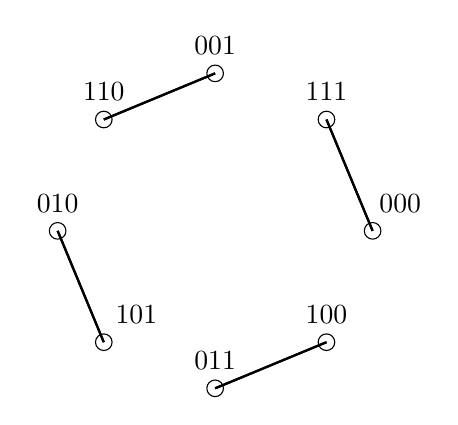
\begin{tikzpicture}
\draw[fill=white] (2.0, 0.0) circle (3pt);
\node at (2.35, 0.35) {000};
\draw[fill=white] (1.414, 1.414) circle (3pt);
\node at (1.414, 1.7639999999999998) {111};
\draw[fill=white] (0.0, 2.0) circle (3pt);
\node at (0.0, 2.35) {001};
\draw[fill=white] (-1.414, 1.414) circle (3pt);
\node at (-1.414, 1.7639999999999998) {110};
\draw[fill=white] (-2.0, 0.0) circle (3pt);
\node at (-2.0, 0.35) {010};
\draw[fill=white] (-1.414, -1.414) circle (3pt);
\node at (-1, -1.064) {101};
\draw[fill=white] (-0.0, -2.0) circle (3pt);
\node at (0.0, -1.65) {011};
\draw[fill=white] (1.414, -1.414) circle (3pt);
\node at (1.414, -1.064) {100};

\draw[thick] (2.0, 0.0) -- (1.414, 1.414);
\draw[thick] (1.414, 1.414) -- (2.0, 0.0);
\draw[thick] (0.0, 2.0) -- (-1.414, 1.414);
\draw[thick] (-1.414, 1.414) -- (0.0, 2.0);
\draw[thick] (-2.0, 0.0) -- (-1.414, -1.414);
\draw[thick] (-1.414, -1.414) -- (-2.0, 0.0);
\draw[thick] (-0.0, -2.0) -- (1.414, -1.414);
\draw[thick] (1.414, -1.414) -- (-0.0, -2.0);
\end{tikzpicture}

\medskip
$S_4$:

\medskip
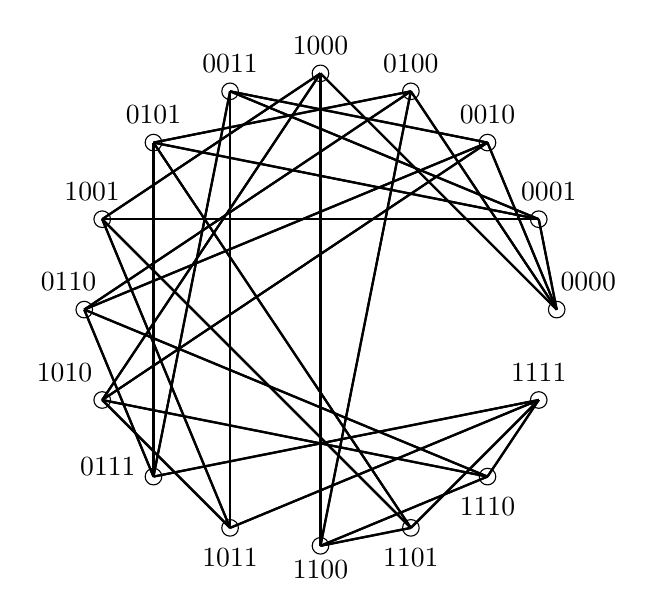
\begin{tikzpicture}
\draw[fill=white] (3.0, 0.0) circle (3pt);
\node at (3.4, 0.35) {0000};
\draw[fill=white] (2.772, 1.148) circle (3pt);
\node at (2.9, 1.4979999999999998) {0001};
\draw[fill=white] (2.121, 2.121) circle (3pt);
\node at (2.121, 2.471) {0010};
\draw[fill=white] (1.148, 2.772) circle (3pt);
\node at (1.148, 3.122) {0100};
\draw[fill=white] (0.0, 3.0) circle (3pt);
\node at (0.0, 3.35) {1000};
\draw[fill=white] (-1.148, 2.772) circle (3pt);
\node at (-1.148, 3.122) {0011};
\draw[fill=white] (-2.121, 2.121) circle (3pt);
\node at (-2.121, 2.471) {0101};
\draw[fill=white] (-2.772, 1.148) circle (3pt);
\node at (-2.9, 1.4979999999999998) {1001};
\draw[fill=white] (-3.0, 0.0) circle (3pt);
\node at (-3.2, 0.35) {0110};
\draw[fill=white] (-2.772, -1.148) circle (3pt);
\node at (-3.25, -0.7979999999999999) {1010};
\draw[fill=white] (-2.121, -2.121) circle (3pt);
\node at (-2.7, -2) {0111};
\draw[fill=white] (-1.148, -2.772) circle (3pt);
\node at (-1.148, -3.15) {1011};
\draw[fill=white] (-0.0, -3.0) circle (3pt);
\node at (0.0, -3.3) {1100};
\draw[fill=white] (1.148, -2.772) circle (3pt);
\node at (1.148, -3.15) {1101};
\draw[fill=white] (2.121, -2.121) circle (3pt);
\node at (2.121, -2.5) {1110};
\draw[fill=white] (2.772, -1.148) circle (3pt);
\node at (2.772, -0.7979999999999999) {1111};

\draw[thick] (3.0, 0.0) -- (2.121, 2.121);
\draw[thick] (3.0, 0.0) -- (2.772, 1.148);
\draw[thick] (3.0, 0.0) -- (0.0, 3.0);
\draw[thick] (3.0, 0.0) -- (1.148, 2.772);
\draw[thick] (2.772, 1.148) -- (3.0, 0.0);
\draw[thick] (2.772, 1.148) -- (-1.148, 2.772);
\draw[thick] (2.772, 1.148) -- (-2.121, 2.121);
\draw[thick] (2.772, 1.148) -- (-2.772, 1.148);
\draw[thick] (2.121, 2.121) -- (3.0, 0.0);
\draw[thick] (2.121, 2.121) -- (-1.148, 2.772);
\draw[thick] (2.121, 2.121) -- (-3.0, 0.0);
\draw[thick] (2.121, 2.121) -- (-2.772, -1.148);
\draw[thick] (1.148, 2.772) -- (3.0, 0.0);
\draw[thick] (1.148, 2.772) -- (-2.121, 2.121);
\draw[thick] (1.148, 2.772) -- (-3.0, 0.0);
\draw[thick] (1.148, 2.772) -- (-0.0, -3.0);
\draw[thick] (0.0, 3.0) -- (3.0, 0.0);
\draw[thick] (0.0, 3.0) -- (-2.772, -1.148);
\draw[thick] (0.0, 3.0) -- (-0.0, -3.0);
\draw[thick] (0.0, 3.0) -- (-2.772, 1.148);
\draw[thick] (-1.148, 2.772) -- (2.121, 2.121);
\draw[thick] (-1.148, 2.772) -- (2.772, 1.148);
\draw[thick] (-1.148, 2.772) -- (-2.121, -2.121);
\draw[thick] (-1.148, 2.772) -- (-1.148, -2.772);
\draw[thick] (-2.121, 2.121) -- (2.772, 1.148);
\draw[thick] (-2.121, 2.121) -- (-2.121, -2.121);
\draw[thick] (-2.121, 2.121) -- (1.148, 2.772);
\draw[thick] (-2.121, 2.121) -- (1.148, -2.772);
\draw[thick] (-2.772, 1.148) -- (-1.148, -2.772);
\draw[thick] (-2.772, 1.148) -- (2.772, 1.148);
\draw[thick] (-2.772, 1.148) -- (0.0, 3.0);
\draw[thick] (-2.772, 1.148) -- (1.148, -2.772);
\draw[thick] (-3.0, 0.0) -- (2.121, 2.121);
\draw[thick] (-3.0, 0.0) -- (2.121, -2.121);
\draw[thick] (-3.0, 0.0) -- (-2.121, -2.121);
\draw[thick] (-3.0, 0.0) -- (1.148, 2.772);
\draw[thick] (-2.772, -1.148) -- (2.121, 2.121);
\draw[thick] (-2.772, -1.148) -- (-1.148, -2.772);
\draw[thick] (-2.772, -1.148) -- (0.0, 3.0);
\draw[thick] (-2.772, -1.148) -- (2.121, -2.121);
\draw[thick] (-2.121, -2.121) -- (-1.148, 2.772);
\draw[thick] (-2.121, -2.121) -- (2.772, -1.148);
\draw[thick] (-2.121, -2.121) -- (-3.0, 0.0);
\draw[thick] (-2.121, -2.121) -- (-2.121, 2.121);
\draw[thick] (-1.148, -2.772) -- (-1.148, 2.772);
\draw[thick] (-1.148, -2.772) -- (2.772, -1.148);
\draw[thick] (-1.148, -2.772) -- (-2.772, -1.148);
\draw[thick] (-1.148, -2.772) -- (-2.772, 1.148);
\draw[thick] (-0.0, -3.0) -- (2.121, -2.121);
\draw[thick] (-0.0, -3.0) -- (0.0, 3.0);
\draw[thick] (-0.0, -3.0) -- (1.148, 2.772);
\draw[thick] (-0.0, -3.0) -- (1.148, -2.772);
\draw[thick] (1.148, -2.772) -- (-0.0, -3.0);
\draw[thick] (1.148, -2.772) -- (-2.121, 2.121);
\draw[thick] (1.148, -2.772) -- (2.772, -1.148);
\draw[thick] (1.148, -2.772) -- (-2.772, 1.148);
\draw[thick] (2.121, -2.121) -- (-0.0, -3.0);
\draw[thick] (2.121, -2.121) -- (2.772, -1.148);
\draw[thick] (2.121, -2.121) -- (-3.0, 0.0);
\draw[thick] (2.121, -2.121) -- (-2.772, -1.148);
\draw[thick] (2.772, -1.148) -- (-1.148, -2.772);
\draw[thick] (2.772, -1.148) -- (2.121, -2.121);
\draw[thick] (2.772, -1.148) -- (-2.121, -2.121);
\draw[thick] (2.772, -1.148) -- (1.148, -2.772);
\end{tikzpicture}


\bigskip
\noindent{\bf 1.29}

\bigskip
\noindent{\bf 1.30}

\bigskip
\noindent{\bf 1.32}

\end{document}